\documentclass{llncs}

\usepackage[utf8]{inputenc}
\usepackage{graphicx}
\usepackage{url}
\usepackage{xspace}
\usepackage{amsmath}
\usepackage{hyperref}
\usepackage[usenames,dvipsnames]{color}
\usepackage{listings}
\newcommand{\CodeSymbol}[1]{\textcolor{Bittersweet}{#1}}
\lstset{
   language=Ada,
   keywordstyle=\color{RedViolet}\ttfamily\bf,
   showspaces=false,
   basicstyle={\scriptsize \sffamily},
   commentstyle=\color{red}\textit,
   stringstyle=\color{MidnightBlue}\ttfamily,
   string=[b]",  % remove ' from string delimiter as it interfers with attributes
   showtabs=false,
   showstringspaces=false,
   morekeywords=[1]Pre,
   morekeywords=[1]Post,
   morekeywords=[1]Test\_Case,
   morekeywords=[1]Contract\_Cases,
   morekeywords=[1]some,
   morekeywords=[1]Old,
   morekeywords=[1]Global,
   morekeywords=[1]Depends,
   morekeywords=[1]Loop\_Invariant,
   morekeywords=[1]Loop\_Variant,
   morekeywords=[1]Loop\_Entry,
   morekeywords=[1]Increases,
   literate={(}{{\CodeSymbol{(}}}1
            {)}{{\CodeSymbol{)}}}1
            {>}{{\CodeSymbol{$>$}}}1
            {>=}{{\CodeSymbol{$\ge$}}}1
            {<}{{\CodeSymbol{$<$}}}1
            {<=}{{\CodeSymbol{$\le$}}}1
            {=}{{\CodeSymbol{$=$}}}1
            {:}{{\CodeSymbol{$:$}}}1
            {.}{{\CodeSymbol{$.$}}}1
            {;}{{\CodeSymbol{$;$}}}1
            {/=}{{\CodeSymbol{$\ne$}}}1
            {=>}{{\CodeSymbol{$\Rightarrow$}}}1
            {->}{{\CodeSymbol{$\rightarrow$}}}1
            {<->}{{\CodeSymbol{$\leftrightarrow$}}}1
}

\newcommand{\DO}{\textsc{do-178}\xspace}
\newcommand{\DOB}{\textsc{do-178b}\xspace}
\newcommand{\DOC}{\textsc{do-178c}\xspace}
\newcommand{\hilite}{Hi-Lite\xspace}
\newcommand{\openetcs}{openETCS\xspace}
\newcommand{\gnatprove}{GNATprove\xspace}
\newcommand{\oldspark}{SPARK~2005\xspace}
\newcommand{\newspark}{SPARK~2014\xspace}
\newcommand{\spark}{SPARK\xspace}
\newcommand{\ada}{Ada\xspace}
\newcommand{\adatwtw}{Ada~2012\xspace}
\newcommand{\altergo}{Alt-Ergo\xspace}

\newcommand{\etc}{\textit{etc.}\xspace}
\newcommand{\ie}{\textit{i.e.}\xspace}
\newcommand{\adhoc}{\textit{ad hoc}\xspace}
\newcommand{\Eg}{\textit{E.g.}\xspace}
\newcommand{\eg}{\textit{e.g.}\xspace}
\newcommand{\etal}{\textit{et al.}\xspace}
\newcommand{\wrt}{w.r.t.\xspace}
\newcommand{\aka}{a.k.a.\xspace}
\newcommand{\resp}{resp.\xspace}

\urlstyle{sf}

\title{Auto-Active Proof of Red-Black Trees in \spark\thanks{Work partly
supported by the Joint Laboratory ProofInUse (ANR-13-LAB3-0007,
\url{http://www.spark-2014.org/proofinuse}) and project VECOLIB
(ANR-14-CE28-0018) of the French national research organization.}}

\author{Claire Dross \and Yannick Moy}
\institute{AdaCore, F-75009 Paris}

\date{}

\begin{document}
\sloppy
\hbadness=9999
\maketitle

\paragraph{Abstract}
Formal program verification can guarantee that a program is free from broad
classes of errors (like reads of uninitialized data and run-time errors) and
that it complies with its specification. Tools such as \spark make it cost
effective to target the former in an industrial context, but the latter is much
less common in industry, owing to the cost of specifying the behavior of
programs and even more the cost of achieving proof of such specifications. We
have chosen in \spark to rely on the techniques of auto-active verification for
providing cost effective formal verification of functional properties. These
techniques consist in providing annotations in the source code that will be
used by automatic provers to complete the proof. To demonstrate
the potential of this approach, we have chosen to formally specify a library
of red-black trees in \spark, and to prove its functionality using auto-active
verification. To the best of our knowledge, this is the most complex use of
auto-active verification so far.

%% \paragraph{Keywords}
%% System formal development, Verification and validation,
%% Certification and dependability

\section{Introduction}

Formal program verification allows programmers to guarantee that the programs
they write have some desired properties. These properties may simply be that
the program does not crash or behave erratically, or more complex critical
properties related to safety or security. Being able to guarantee such
properties will be essential for high assurance software as requirements are
increasingly complex and security attacks more pervasive.

SPARK is a subset of the Ada programming language targeted at safety- and
security-critical applications. GNATprove is a tool that analyzes SPARK code
and can prove absence of run-time errors and user-specified properties
expressed as contracts. GNATprove is based on modular deductive verification of
programs, analyzing each function in isolation based on its contract and the
contracts of the functions it calls. The main benefit of this approach is that
it allows using very precise semantics of programming constructs and powerful
automatic provers. The main drawback is that top-level specifications are not
sufficient. Programmers need to provide many intermediate specifications in the
form of additional contracts, loop invariants and assertions.

Providing the right intermediate specifications is a difficult art, but
progress has been achieved in recent years through a method known as
auto-active verification. Various languages and tools now provide
features for effective auto-active verification. SPARK is among
these. In this paper, we explore the capabilities of auto-active verification
for automatically proving complex algorithms. We have chosen to target
red-black trees because they are well-known, commonly used in practice, and yet
sufficiently complex that no implementation of imperative red-black trees has
been formally verified using auto-active verification. Our implementation of
red-black trees, with all the code for auto-active verification, is publicly
available in the repository of
SPARK.~\footnote{\url{https://github.com/AdaCore/spark2014/tree/master/testsuite/gnatprove/tests/red_black_trees}}


% implem available on github

%% \spark is a subset of the Ada programming language targeted at safety- and
%% security-critical applications. \spark formal verification toolset allows to
%% guarantee that a \spark program is free from broad classes of errors (like reads
%% of uninitialized data and run-time errors) and that it complies with its
%% specification. While the former is a well adopted practice among \spark users,
%% the latter is used much more narrowly, owing to the cost of specifying the
%% behavior of programs and even more the cost of achieving proof of such
%% specifications. \spark relies on automatic provers to keep the cost of formal
%% verification reasonable, and on the techniques of auto-active verification for
%% interacting with automatic provers. In this paper, we present how we applied
%% auto-active verification to formally verify a library of red-black trees. To
%% the best of our knowledge, this is the most advanced use of auto-active
%% verification so far.

\section{Preliminaries}
\subsection{\spark 2014}

\spark is a subset of the Ada programming language targeted at safety-
and security-critical applications. \spark builds on the strengths of
Ada for creating highly reliable and long-lived software. \spark
restrictions ensure that the behavior of a \spark program is
unambiguously defined, and simple enough that formal verification
tools can perform an automatic diagnosis of conformance between a
program specification and its implementation. The \spark language and
toolset for formal verification have been applied over many years to
on-board aircraft systems, control systems, cryptographic systems, and
rail systems~\cite{oneill2012}.

In the versions of \spark up to \spark 2005, specifications are written as
special annotations in comments. Since version \spark 2014~\cite{mccormick15},
specifications are written as special Ada constructs attached to
declarations. In particular, various contracts can be attached to subprograms:
data flow contracts, information flow contracts, and functional contracts
(preconditions and postconditions, introduced respectively by \texttt{Pre} and
\texttt{Post}). An important difference between \spark 2005 and \spark 2014 is
that functional contracts are executable in \spark 2014, which greatly
facilitates the combination of test and proof. The definition of the
language subset is motivated by the simplicity and feasibility of formal
analysis and the need for an unambiguous semantics. Tools are available that
provide flow analysis and proof of \spark programs.

Flow analysis checks correct access to data in the program: correct access to
global variables (as specified in data and information flow contracts) and
correct access to initialized data. Proof is used to demonstrate that the
program is free from run-time errors such as arithmetic overflow, buffer
overflow and division-by-zero, and that the functional contracts are correctly
implemented. \gnatprove is the tool implementing both flow analysis and proof
of SPARK code.

\subsection{Auto-active Verification}
\label{sec-prelim-auto-active}

The term \emph{auto-active verification} was coined in 2010 by researcher
Rustan Leino~\cite{Leino10usableauto-active} to characterise \textit{tools where
  user input is supplied before VC generation [and] therefore lie between
  automatic and interactive verification} (hence the name auto-active). This is
in contrast to fully automatic verifiers for which \textit{the specification is
  fixed} and interactive verifiers for which \textit{the user input is supplied
  after VC generation, which is the typical case when the reasoning engine is
  an interactive proof assistant}. Auto-active verification is at the center of
the academic formal program verification toolsets Dafny~\cite{Leino2010Dafny},
the Eiffel Verification Environment (EVE)~\cite{Furia2016},
Why3~\cite{filliatre2013Why3} as well as the industrial formal program
verification toolsets Frama-C~\footnote{\url{http://frama-c.com/}} and
\spark~\footnote{\url{http://www.adacore.com/sparkpro/}}.

In all these toolsets, auto-active verification consists in a set of
specification features at the level of the source language, and a set of tool
capabilities to interact with users at the level of the source code. The
specification features consist at least in constructs to specify function
contracts (preconditions and postconditions) and data invariants, as well as
specialized forms of assertions (loop invariants and loop variants, assumptions
and assertions). All the toolsets mentioned above also support \emph{ghost code},
a feature to instrument code for verification. Ghost
functions are also called lemmas when their main purpose is to support the
proof of a property that is later used at the point where the function is
called. See \cite{kosmatov:hal-01344110} for a comparison of how ghost code
differs between Why3, Frama-C and \spark. Various tool capabilities facilitate
user interaction at source level: fast running time that exploits
multiprocessor architectures and minimizes rework between runs, the ability to
trade running time for more verification power, feedback from the toolset when
verification is unsuccessful (counterexamples in particular).

Auto-active verification in the above toolsets has been used to fully verify
algorithms, libraries and even full applications: examples include a
container library in Eiffel~\cite{Polikarpova2015}, distributed systems in
Dafny~\cite{Hawblitzel2015IronFleet}, secure execution of apps in
Dafny~\cite{Hawblitzel2014Ironclad}, binary heaps in Why3~\cite{tafat11rr},
allocators in \spark~\cite{Dross2016}.

\subsection{Red-Black Trees}
\label{sec-prelim-rbt}

Red-black trees are a kind of self-balancing binary search trees. Nodes in the
tree are colored red or black, and balance is maintained by ensuring that two
properties are preserved: (1)~a red node can only have black children, and
(2)~every path from the root to a leaf has the same number of black nodes. The
consequence of these two properties is that the path from the root to a leaf
can be at most twice as long as the path from the root to another leaf.

Implementations of red-black trees are used in the Linux kernel (in C) and
standard container libraries for various languages (C++ STL, Java.util,
Ada). The insertion and deletion algorithms work by inserting or deleting the
node as in a binary search tree, which may violate properties~(1) and~(2)
above, and then restoring the balance by working their way up on the path from
the root to the point of insertion or deletion. At every node on this path, the
algorithms may \emph{rotate} the subtree, which consists in a local
rearrangement of nodes to restore properties~(1) and~(2). These algorithms are
sufficiently complex that no implementation of imperative red-black trees has
been formally verified in Dafny, Eiffel or Why3. See
Section~\ref{related-work} for a list of the closest works, including some
using auto-active verification. We are following the algorithm from Cormen et
al.~\cite{Cormen2009} for insertion in a red-black tree. We did not implement
the deletion algorithm, which would be very similar to insertion. In the same
way, we did not verify that every branch in a red-black tree contains the same
number of black nodes.

\section{Red-Black Trees in \spark}
\subsection{Invariants and Models}
\label{sec-rbt-inv}
% invariants of data structures
% relation between invariants and models
% public model of RBT
% internal model of tree

% hierarchy done with proof in mind, separation of concerns
%    binary_trees => tree structure
%    search_trees => ordered values
%    red_black_trees => balanceness
% properties stored in (private) invariants and reflected in (public) models
%    binary_trees => reachability
%    search_trees => set of contained values
%    red_black_trees => no model
% models should be easy to use/complex to verify to factor complexity
%  ex: provide a model of reachability
% primitives needed by upper levels provided at lower level were they abide by the invariant

Implementing red-black trees correctly from the algorithm is straightforward,
but this implementation is hard to verify formally, as it forces one to
reason about different levels of properties all at once. Instead, we have
divided the implementation into three distinct parts, each one concerned with
one property level: binary trees, search trees and red-black trees. Binary
trees maintain a tree structure on the underlying memory. Search trees build on
binary trees by associating values to tree nodes and maintain the order of
values in the tree. Red-black trees build on search trees and enforce balancing
using the classical red-black tree coloring mechanism.

The property enforced at each level is expressed in a type invariant. In SPARK,
the invariant may be temporarily violated inside the implementation of the
functions that operate on the type, but are guaranteed to hold for external
users of objects of that type. More precisely, functions that operate
on a type can assume the invariant on entry and must restore it on exit (which
leads to verification conditions in SPARK).
%%  while internal functions need not
%% assume nor restore the invariant. The invariant must also be restored for any
%% parameter or global variable that is an input of a possibly reentrant call
%% (which also leads to verification conditions in SPARK). At each level, the type
%% invariant supports the proof of postconditions for functions that operate on
%% the type.

\paragraph{Binary trees:}
As explained in Section~\ref{sec-implementation}, binary trees are
implemented as arrays, using the representation described in Figure~\ref{fig-binary}.
Each node contains a reference to its left and right children, if any, as well
as a reference to its parent and a position, which may be Top for the root,
Right or Left otherwise depending on the node position with respect to its
parent. The invariant of binary trees states that values of these fields are
consistent across the tree. For example, the left child of a node has position
Left and the node as parent.

\begin{figure}[ht]
\begin{center}
%\hrulefill
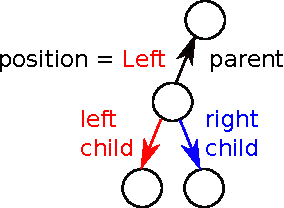
\includegraphics[width=4cm]{tree_structure.pdf}\hfill
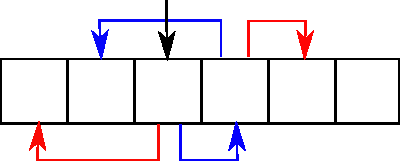
\includegraphics[width=5cm]{binary_1.pdf}\hfill
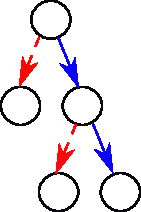
\includegraphics[width=2cm]{binary_2.pdf}
\caption{(from left to right) Representation of nodes in binary trees.
Example of a binary tree, for readability, parents and positions are not represented.
A higher level view of the same binary tree.}
%\hrulefill
%\vspace*{-10mm}
\label{fig-binary}
\end{center}
\end{figure}

%% \begin{figure}[ht]
%% \begin{small}
%% \begin{lstlisting}
%% -- If a cell is the root of a tree (position Top) it has no parent
%% (for all I in Index_Type =>
%%    (if Position (I) = Top then Parent (I) = Empty))

%% -- If a cell I has a left child, then its left child has position
%% -- Left and parent I.
%% and then (for all I in Index_Type =>
%%            (if Left (I) /= Empty then
%%               Position (Left (I)) = Left and Parent (Left (I)) = I))

%% -- If a cell I has a right child, then its right child has position
%% -- Right and parent I.
%% and then (for all I in Index_Type =>
%%            (if Right (I) /= Empty then
%%              Position (Right (I)) = Right and Parent (Right (I)) = I))

%% -- If a cell is a child (position Left or Right), then it is the
%% -- child of its parent.
%% and then (for all I in Index_Type =>
%%            (if Position (I) = Left then Left (Parent (I)) = I))
%% and then (for all I in Index_Type =>
%%            (if Position (I) = Right then Right (Parent (I)) = I))
%% \end{lstlisting}
%% \end{small}
%% \caption{\label{fig-binary-inv} Type invariant of binary trees.}
%% \end{figure}
% Do we want to write Position (F, I) instead of Position (I)?

To reason about the tree structure at a higher level, we provide a model of binary trees
which makes explicit the
\emph{access paths} from the root to every node in the tree.
% Contrary to the invariant,
% the model needs to be visible outside of the implementation of binary trees, in
% order to express more complex properties.
It associates a sequence of
directions, namely Right or Left, with each node in the binary tree,
corresponding to the path from the root to the node. As the underlying array
also contains unused cells that do not correspond to tree nodes, an additional
boolean encodes whether the node belongs to the
tree. Figure~\ref{fig-binary-mod-ex} gives the model of the binary tree
presented in Figure~\ref{fig-binary}. In this example, all the nodes belong to
the tree except the last one. The access paths written below each node can be used to
reconstruct easily the high level view of the tree.

% We define a function \texttt{Model} that
% returns the model of a binary tree. This function has a rich postcondition that
% uniquely defines the model. The access path of the root is empty and the access path of other nodes is
% computed from the access path of their parent. Proof of the function \texttt{Model}
% relies on the invariant over binary trees. Its definition
% is then available for users of binary trees who can call function
% \texttt{Model} to express complex properties over the structure.

%% As an example, reachability in the tree structure is a complex property, that is
%% crucial to reason about search trees. Reachability is difficult to tackle for \spark
%% as it is an inductive porperty, and therefore requires inductive proofs. To factor out
%% this complexity at the binary tree level, we introduce
%% a model of binary trees allowing to reason easily about branches in the tree, see
%% Figure~\ref{fig-binary-mod}.

%% \begin{figure}[ht]
%% \begin{small}
%% \begin{lstlisting}
%% type Position_Type is (Left, Right, Top);
%% subtype Direction is Position_Type range Left .. Right;

%% package D_Seq is new Conts.Functional.Sequences
%%   (Positive_Count_Type, Direction);
%% use D_Seq;
%% --  Sequence of directions modelling a path from the root of the tree
%% --  to a node in the tree.

%% type Path_Type is record
%%    A : Sequence;
%%    K : Boolean := False;
%% end record
%% with Predicate => Length (A) <= Max;
%% --  Type used to model the path from the root of a tree to a given,
%% --  node which may or not be in the tree:
%% --    - if a node is in the tree, the corresponding path will have K =
%% --      True, and A will denote the path from the root to this node.
%% --    - if a node is not in the tree, the corresponding path will have
%% --      K = False and A will be empty.
%% \end{lstlisting}
%% \end{small}
%% \caption{\label{fig-binary-mod} Model of branches in a binary tree.}
%% \end{figure}


\begin{figure}[ht]
\begin{center}
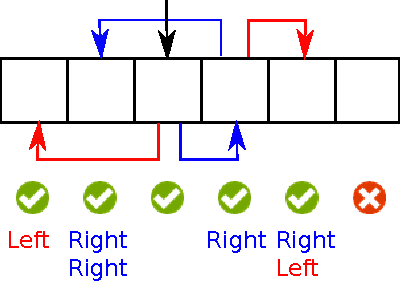
\includegraphics[width=5cm]{model.pdf}
\caption{\label{fig-binary-mod-ex} Example of model of a binary tree.}
\end{center}
\end{figure}

%% Only valid binary trees are associated a model, that is, the model function
%% only works on trees for which the tree structure invariant holds. As a result,
%% we cannot use this model function inside the implemenation of binary tree,
%% for example to state in the invariant that all the nodes are reachable from the
%% root (there is no memory leak). However, as type invariants always hold outside
%% the data structures implementations, the path model can safely be used for any
%% binary tree in the implementation of search trees. In particular, we use it
%% in the invariant of search trees, which is given in Figure~\ref{fig-search}.

\vspace{-1cm}
\begin{figure}[ht]
\hspace{-3mm}
\begin{minipage}[c]{.79\linewidth}
\begin{small}
\begin{lstlisting}
(for all I in Index_Type =>
  (for all J in Index_Type =>
    (if Model (T) (I).Reachable
      and Model (T) (J).Reachable
      and Model (T) (I).Path < Model (T) (J).Path
     then (if Get (Model (T) (J).Path,
                   Length (Model (T) (I).Path) + 1) = Left
           then Values (J) < Values (I)
           else Values (J) > Values (I)))))
\end{lstlisting}
\end{small}
\end{minipage}
\begin{minipage}[c]{.22\linewidth}
\begin{center}
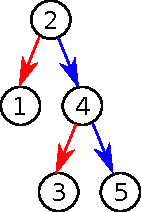
\includegraphics[width=2cm]{search.pdf}
\end{center}
\end{minipage}
\caption{\label{fig-search} Type invariant of search trees. For a search tree \texttt{T},
\texttt{Model (T)} returns the model of the underlying binary tree of \texttt{T}.
For each index \texttt{I} in the underlying
array, if \texttt{Model (T) (I).Reachable} is true then \texttt{I} is reachable
in \texttt{T} and \texttt{Model (T) (I).Path} is the sequence
of directions corresponding to the path from the root of \texttt{T} to \texttt{I}.
$<$ stands for prefix order on paths.}
\end{figure}

\paragraph{Search trees:}
The invariant of search trees states that the value stored in each node of the
tree is larger than all the values stored in the subtree rooted at its left
child and smaller than all the values stored in the subtree rooted at its right
child. It is given in Figure~\ref{fig-search}, together with an example of values that would
fit the tree from Figure~\ref{fig-binary}. To express this invariant, we use the model of the
underlying binary tree. The value stored at node \texttt{J} belonging to the subtree
rooted at node \texttt{I} (where path inclusion from the root is used to determine that
\texttt{J} belongs to the subtree rooted at node \texttt{I}) is smaller (resp. greater) than the
value stored at node \texttt{I} if \texttt{J} belongs to the subtree rooted at the left
(resp. right) child of \texttt{I}.

\paragraph{Red-black trees:}
The invariant of red-black trees states that a red node can only have black
children. It is given in Figure~\ref{fig-rbt}. An example of colors that would
fit the tree from Figure~\ref{fig-search} is also given in
Figure~\ref{fig-rbt}.  This corresponds to property~(1) of red-black trees as
presented in Section~\ref{sec-prelim-rbt}. Verifying property~(2) would require
implementing a new inductive model function over binary trees, like the one we
defined for reachability. As it would be very similar to the work presented
here, and would essentially double the effort, we did not attempt it.

%% Finally, the last level of our tree implementation is concerned with balancanceness.
%% As explained in Section~\ref{sec-prelim-rbt}, each node is colored either black or red
%% and invariants are maintained to ensure that the longest branch in the tree is at most
%% twice as long as the shortest branch. Figure~\ref{fig-rbt} demonstrates a coloring of
%% the tree from Figure~\ref{fig-search}.

\begin{figure}[ht]
\begin{minipage}[c]{.77\linewidth}
\begin{small}
\begin{lstlisting}
(for all I in Index_Type =>
   (if Parent (T.Struct, I) = Empty
      or else T.Color (Parent (T.Struct, I)) = Red
    then T.Color (I) = Black))
\end{lstlisting}
\end{small}
\end{minipage}\hfill
\begin{minipage}[c]{.22\linewidth}
\begin{center}
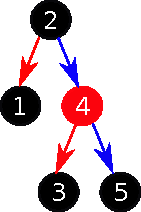
\includegraphics[width=2cm]{red_black.pdf}
\end{center}
\end{minipage}
\caption{\label{fig-rbt} Type invariant of red-black trees.}
\end{figure}

\subsection{Implementation}
\label{sec-implementation}
% no pointer in spark => indexes inside an array
% avoid copies, use forest
% it is bounded
% values and colors are outside, in separate array (to avoid having them in the frame)
% provide plug/extract to modify the forest while keeping the invariant
% rotate_left and rotate_right preserve the order

Our implementation of red-black trees differs on two accounts from the
straighforward implementation of the algorithm. First, as stated above,
we used an array as the
underlying memory for trees, instead of dynamically allocating nodes. This is
to comply with a restriction of SPARK which does not allow pointers, but only
references and addresses. The rationale for this restriction is that pointers
make automatic proof very difficult due to possible aliasing. Hence trees are
bounded by the size of the underlying array. As the algorithm for balancing
red-black trees requires splitting and merging trees, we had the choice of
either copying arrays for generating new trees, or sharing the same array
between disjoint trees (coming from the splitting of a unique tree). For
obvious efficiency reasons, we chose the latter. Hence we are defining a type
\texttt{Forest} for possibly representing disjoint binary trees sharing the
same underlying array.

%% Note that we are dealing everywhere with forests of binary trees instead of a single
%% binary tree. This is because, as we are using arrays instead of pointers, we cannot divide a
%% tree object into separate objects without copying the array around. To keep an efficient
%% implementation, we resorted to processing the memory region as a whole, therefore
%% introducing forests of trees, in which every allocated node with a \texttt{Top} position is a
%% valid root.

%% From a software verification perspective, it may seem strange to present the implementation
%% before the specification. Here we do so because the implementation is comparatively
%% simpler and more widely known than the specification. And indeed, our implementation
%% resemble standard imperative implementations of red-black trees except for two notable
%% points. The first one is that we had to comply with the restrictions imposed by the
%% \spark language, most notably, the forbidding of pointers (access types in Ada). To
%% alleviate this restriction, we chose to implement binary trees inside an array, indexes
%% working as pointers in a memory region. To simplify our implementation, we do not consider
%% node deallocation, so that unallocated cells are located after a given index in the array.
%% The Ada type of binary trees is given in Figure~\ref{fig-binary-typ}.
%% Note that our trees are bounded by the size of the underlying array.

%% \begin{figure}[ht]
%% \begin{small}
%% \begin{lstlisting}
%% type Cell is record
%%    Left, Right, Parent : Extended_Index_Type := Empty;
%%    Position            : Position_Type := Top;
%% end record;
%% type Cell_Array is array (Index_Type) of Cell;

%% type Forest is record
%%    S : Extended_Index_Type := Empty;
%%    C : Cell_Array;
%% end record
%%   with Type_Invariant => Tree_Structure (Forest);
%% --  Component S gives the size of the forest. Only the cells up to
%% --  index S belong to the forest. Cells after index S are free.
%% \end{lstlisting}
%% \end{small}
%% \caption{\label{fig-binary-typ} Implementation of binary trees.}
%% \end{figure}

%% The other specificity of our implementation is of course the layered design. Since we
%% have chosen to associate a type invariant to binary trees, the \texttt{Forest} type is defined as
%% a private type and it can only be modified by users using functions which abide by the
%% invariant. Therefore, we cannot change the values of the \texttt{Cell} record components individually
%% from outside of binary trees implementation. We have resorted to defining functions
%% doing single modifications of the tree while preserving the invariant. The modification
%% functions provided for binary trees are given in Figure~\ref{fig-binary-fun}.

The other distinguishing feature of our implementation is the layered design. Each module
defining a type with an invariant also needs to provide functions for
manipulating objects of the type while preserving their invariant. As an example,
binary trees are not updated by direct assignments in the implementation of search
trees, but using two new functions, \texttt{Extract} and
\texttt{Plug}, which split and merge disjoint trees while preserving the forest invariant.

% \begin{figure}[ht]
% \begin{minipage}[c]{.75\linewidth}
% \begin{small}
% \begin{lstlisting}
% procedure Extract (F    : in out Forest;
%                    R, I : Index_Type;
%                    D    : Direction;
%                    V    : out Extended_Index_Type);
% -- Extract the subtree starting at position D after
% -- I in the tree rooted at R in a separate tree.
% -- Store its root into V.
%
% procedure Plug (F    : in out Forest;
%                 R, I : Index_Type;
%                 D    : Direction;
%                 V    : Extended_Index_Type);
% -- Plug the tree rooted at V in F into the tree
% -- rooted at R as a subtree starting at position D
% -- after I.
% \end{lstlisting}
% % \end{lstlisting}
% \end{small}
% \end{minipage} \hfill
% \begin{minipage}[c]{.23\linewidth}
% 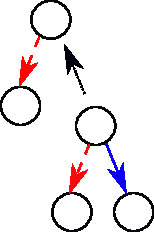
\includegraphics[width=2cm]{plug.pdf}
% \end{minipage}
% \caption{\label{fig-binary-fun} Functions on binary trees.}
% \end{figure}

%% As type invariants can be temporarily broken inside the data structure implementation, the body
%% of the modification functions can directly modify the internal structure of the tree. The implementation
%% of \texttt{Plug} is presented in Figure~\ref{fig-binary-body}.

%% \begin{figure}[ht]
%% \begin{small}
%% \begin{lstlisting}
%% procedure Plug (F    : in out Forest;
%%                 R, I : Index_Type;
%%                 D    : Direction;
%%                 V    : Extended_Index_Type) is
%% begin
%%    if V /= Empty then
%%       if D = Left then
%%          F.C (I).Left := V;
%%       else
%%          F.C (I).Right := V;
%%       end if;

%%       F.C (V).Position := D;
%%       F.C (V).Parent := I;
%%    end if;
%% end Plug;
%% \end{lstlisting}
%% \end{small}
%% \caption{\label{fig-binary-body} Implementation of \texttt{Plug}.}
%% \end{figure}

At the next layer, search trees are defined as binary trees along with an
additional array of values. As we only need to consider complete search trees,
the underlying forest needs to only hold one tree, which is identified through
its root. The module defining search trees provides basic set functions, namely
inserting a value into the tree and testing a value for membership in the
tree. It also provides balancing functions for the upper layer of red-black
trees. They allow rotating nodes of a search tree to the left or to the right
while preserving the order between values. An example of such a rotation is
given in Figure~\ref{fig-search-rot}.  Defining these balancing functions
inside the implementation of search trees rather than inside the implementation
of red-black trees allows keeping all order-related concerns in the search tree
layer. Indeed, balancing functions do not preserve balance, as they are to be
called on unbalanced trees, but they do preserve order. Note that implementing
the balancing functions at this level avoids the need for lifting low-level
tree handling functions such as \texttt{Plug} and \texttt{Extract} at the next
layer. All the functions defined on search trees are implemented using
functions over binary trees.

%% Following our leveled approach, search trees are defined outside of binary tree implementation.
%% They are binary trees along with an additional array of values. Also, as we never need to consider
%% parts of search trees, we no longer work on complete forests but rather on a single tree. More
%% precisely, we store a single root index in the search tree data structure.
%% The Ada type of search trees is given in Figure~\ref{fig-search-typ}.

%% \begin{figure}[ht]
%% \begin{small}
%% \begin{lstlisting}
%% type Value_Array is array (Index_Type) of Natural;

%% type Search_Tree is record
%%    Root   : Extended_Index_Type := Empty;
%%    Struct : Forest;
%%    Values : Value_Array := (others => 0);
%% end record
%%   with Type_Invariant => ...;
%% \end{lstlisting}
%% \end{small}
%% \caption{\label{fig-search-typ} Implementation of search trees.}
%% \end{figure}

\begin{figure}[ht]
\begin{center}
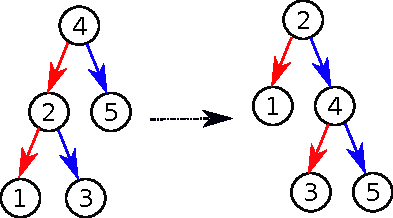
\includegraphics[width=5cm]{rotate_right.pdf}
\caption{\label{fig-search-rot} Example of application of Right\_Rotate.}
\end{center}
\end{figure}

Red-black trees are implemented in the same way as search trees by adding an
array of colors to a search tree and using balancing functions to rebalance the
tree after an insertion.

\subsection{Specification}
% use parent/position and model
% model can be derived from parent and position but have it in post to do inductive proofs only once
% invariant about no memory leak derived from post
% - of binary trees: we never have ill formed cyclic trees
% - of search trees: all cells remain accessible from the root

Functional specifications of the insertion and membership functions that operate on
red-black trees consist in simple contracts (preconditions and postconditions)
presented in Figure~\ref{fig-rbt-spec}. These contracts use a model function
\texttt{Values} that returns the set of values in the tree. \texttt{Mem} returns
true if and only if the element is in the tree and \texttt{Insert} adds a new element
in the tree.

%% In this example, we concentrate on functional requirements of two kinds. The most important one is the
%% preservation of the data structure invariants. As a proof of concept, we have also considered
%% function specific requirements, describing the effect of the insertion and membership functions with
%% respect to the set of values contained in the red-black tree. The function specific requirements are the
%% simplest. They are expressed as contracts on the tree functions. The set of values contains in a red-black
%% tree is accessed using a specific model function named \texttt{Values} defined at the search tree level.
%% These contracts are presented in Figure~\ref{fig-rbt-spec}.

\begin{figure}[ht]
\begin{small}
\begin{lstlisting}
function Values (T : Rbt) return Value_Set with
  Post => (if Size (T) = 0 then Is_Empty (Values'Result));

function Mem (T : Rbt; V : Natural) return Boolean with
  Post => Mem'Result = Mem (Values (T), V);

procedure Insert (T : in out Rbt; V : Natural) with
  Pre  => Size (T) < Max,
  Post => (if Mem (T'Old, V) then Values (T) = Values (T'Old)
           else Is_Add (Values (T'Old), V, Values (T)));
\end{lstlisting}
\end{small}
\caption{\label{fig-rbt-spec} Specification of red-black trees.}
\end{figure}

The most complex specifications have to do with the four properties to maintain
over red-black trees:
\begin{enumerate}
 \item A red-black tree is always a valid binary tree (we can navigate it from
   the root in the expected way).
 \item There is no memory leak (if we have inserted fewer than \texttt{Max}
   elements, there is still room enough in the data structure to insert a new
   element).
 \item The values stored in the tree are ordered (it is a valid search tree).
 \item The tree stays balanced (we only verify this property partially, that is, that red
   nodes can only have black children).
\end{enumerate}

As already discussed, each property is specified at the most appropriate layer.
The first property is enforced at the level of binary trees. The invariant on
binary trees (see Section~\ref{sec-rbt-inv}) ensures that the fields of a node
(Parent, Position, Left, and Right) are consistent. This is not enough to
ensure that all the allocated nodes in the forest belong to well-formed binary
trees though, as it does not rule out degenerate, root-less, cyclic structures
that would arise from linking the root of a binary tree as the child of one of
its leafs. Still, this is enough to ensure that red-black trees are always well
formed, as red-black trees always have a root. Note that the fact that every
node in the forest is part of a well formed binary tree is ensured at the level
of binary trees by enforcing that such degenerate structures can never be
created in the contracts of functions operating on binary trees.

The second property is enforced at the level of search trees. It is specified
as a postcondition of every function operating on search trees.
Figure~\ref{fig-spec-no-leak} shows the part of the postcondition of
\texttt{Right\_Rotate} ensuring that it has not introduced any dangling
node. It uses the function \texttt{Model} described in
Section~\ref{sec-rbt-inv} to reason about node reachability.

\begin{figure}[ht]
\begin{small}
\begin{lstlisting}
procedure Right_Rotate (T : in out Search_Tree; I : Index_Type) with
  Post =>
    --  The size of the tree is preserved
    Size (T) = Size (T)'Old

    --  Nodes in the tree are preserved
    and (for all J in Index_Type =>
          Model (T) (J).Reachable = Model (T'Old) (J).Reachable);
\end{lstlisting}
\end{small}
\caption{\label{fig-spec-no-leak} Postcondition of \texttt{Right\_Rotate} dealing with absence of memory leaks.}
\end{figure}

The third and fourth properties are expressed in the type invariant of
respectively search trees and red-black trees as explained in
Section~\ref{sec-rbt-inv}.

Apart from these top-level specifications, many more specifications are needed
on subprograms at lower layers (binary trees and search trees) in order to be
able to prove the properties at higher layers (respectively search trees and
red-black trees). This is inherent to the modular style of verification
supported by \gnatprove. For example, as \texttt{Right\_Rotate} on search trees
calls \texttt{Plug} and \texttt{Extract} on binary trees, the contracts for
these functions need to provide enough information to verify both the absence
of memory leaks as stated in the postcondition of \texttt{Right\_Rotate} and
the preservation of the order of values as stated in the invariant of search
trees.

%% A part of the postcondition of \texttt{Plug} is given in
%% Figure~\ref{fig-spec-binary}.

%% \begin{figure}
%% \begin{small}
%% \begin{lstlisting}
%% procedure Plug (F    : in out Forest;
%%                 R, I : Index_Type;
%%                 D    : Direction;
%%                 V    : Extended_Index_Type)
%%    --  Plug the tree rooted at V in F into the tree rooted at R as a
%%    --  subtree starting at position D after I.

%% with
%%   Pre  => ...,
%%   Post =>
%%     --  The size of the forest does not change
%%     Size (F) = Size (F'Old)

%%     --  V is inserted in the tree as child D of I
%%     and (if D = Left then V = Left (F, I) else V = Right (F, I))

%%     --  Except for V, the value of parent link is preserved
%%     and (for all J in Index_Type =>
%%           (if J /= V then Parent (F, J) = Parent (F'Old, J)))

%%     --  Except for V, the value of position is preserved for nodes which have
%%     --  a parent.
%%     and (for all J in Index_Type =>
%%           (if J /= V then Position (F, J) = Position (F'Old, J)))

%%     --  Nodes in the tree rooted at R come either from the tree previously
%%     --  rooted at R, or for those nodes which have V on their path, from
%%     --  the tree previously rooted at V.
%%     and (for all I in Index_Type =>
%%           (if Model (F, R) (I).Reachable then
%%             (if V /= Empty and Model (F, R) (V).Path <= Model (F, R) (I).Path
%%              then Model (F'Old, V) (I).Reachable
%%              else Model (F'Old, R) (I).Reachable)))

%%     --  Paths are preserved for nodes that were previously in the tree
%%     and (for all J in Index_Type =>
%%           (if Model (F'Old, R) (J).Reachable
%%            then Model (F, R) (J).Path = Model (F'Old, R) (J).Path))

%%     --  The path for nodes in the tree previously rooted at V is obtained
%%     --  by concatenating the path from R to V and the path from V to the
%%     --  node.
%%     and (for all J in Index_Type =>
%%           (if V /= Empty and then Model (F'Old, V) (J).Reachable
%%            then Is_Concat (Left   => Model (F, R) (V).Path,
%%                            Right  => Model (F'Old, V) (J).Path,
%%                            Result => Model (F, R) (J).Path)));
%% \end{lstlisting}
%% \end{small}
%% \caption{\label{fig-spec-binary} Contract of Plug.}
%% \end{figure}

%% The postcondition of \texttt{Plug} describes how it modifies the tree structure. Theoretically,
%% describing how \texttt{Parent} and \texttt{Position} fields are updated by the call should be enough to
%% describe the effect on the whole structure. Still, to avoid having to redo complex
%% proofs each time \texttt{Plug} is call, we choose to also describe the effect of the modification
%% of \texttt{Model}. This allows to clearly separate concerns and allow
%% the implementation of search trees to only concentrate on order related issues.

\subsection{Proof Principles}
% principle of inductive proofs on size of path
% principles of dealing with the frame condition: unmodified trees in forest

% reachability requires proof by induction on the size of the path
%   This is done using loops and loop invariants
% order requires case split
%   This is done using if statements

Verifying our implementation of red-black trees has proved to be challenging,
and above the purely automatic proving capabilities of \gnatprove. There
are several reasons for this:

\begin{itemize}
 \item The imperative, pointer-based implementation of red-black trees makes it difficult
 to reason about disjointness of different trees/subtrees in the forest.
 \item Reasoning about reachability in the tree structure involves inductive proofs, which
 automatic provers are notoriously bad at.
 \item Reasoning about value ordering involves using transitivity relations, that is, coming
 up with an intermediate value to consider, which usually eludes automatic provers.
 \item The size of the formulas to verify, number of verification conditions, and number of
 paths in the program are large enough to defy provers scalability.
\end{itemize}

To work around these limitations, we used auto-active verification techniques, which,
as described in Section~\ref{sec-prelim-auto-active}, can guide automatic provers without
requiring a proof assistant. We explain some of these techniques in this section.

\paragraph{Intermediate lemmas:}
One of the classical techniques in manual proof consists in factoring some useful
part of a proof in an intermediate lemma so that it can be verified independently and
used as many times as necessary. In auto-active verification, this can be done by introducing
a procedure with no output, which, when called, will cause the deductive engine to verify
its precondition and assume its postcondition. In Figure~\ref{fig-proof-lem}, we show an
intermediate lemma which can be used to verify that two trees of a single forest with different
roots are disjoint. A caller of this function will have to verify that \texttt{T1} and \texttt{T2} are different
valid roots in \texttt{F} and as a consequence we know that there can be no node reachable from both roots in \texttt{F}.
Naturally, the lemma is not assumed, its actual proof is performed when verifying the procedure
\texttt{Prove\_Model\_Distinct}.

\begin{figure}
\begin{small}
\begin{lstlisting}
procedure Prove_Model_Distinct (F : Forest; T1, T2 : Index_Type) with
--  Trees rooted at different indexes in the forest are disjoint.
  Pre  => T1 /= T2
    and then Valid_Root (F, T1)
    and then Valid_Root (F, T2),
  Post => (for all I in Index_Type =>
            (not Model (F, T1) (I).Reachable
               or not Model (F, T2) (I).Reachable));
\end{lstlisting}
\end{small}
\caption{\label{fig-proof-lem} Intermediate lemma stating disjointness of trees in a forest.}
\end{figure}

\paragraph{Reasoning by induction:}
Though some automatic provers are able to discharge simple inductive proofs, inductive reasoning
still requires manual interaction in most cases. In auto-active style, an inductive proof can be done
using loop invariants. \gnatprove splits the
verification of a loop invariant in two parts. First, it verifies that the invariant holds in the first iteration of the
loop and then that it holds in any following iteration knowing that it held in the previous one.
This behavior is exactly what we want for a proof by induction. For example, Figure~\ref{fig-proof-ind}
demonstrates how the intermediate lemma presented in Figure~\ref{fig-proof-lem} can be verified
using a loop to perform an induction over the size of the path from the root \texttt{T1} to any node reachable
from \texttt{T1} in \texttt{F}. The loop goes from 1 to the maximum size of any branch
in the forest \texttt{F}. We have written the property we wanted to prove as a loop invariant. To verify this procedure, \gnatprove will
first check that the invariant holds in the first iteration of the loop, that is, that \texttt{T1} itself cannot
be reached from \texttt{T2}. Then, it will proceed by induction to show that this holds for any node reachable
from \texttt{T1} in \texttt{F}.

\begin{figure}
\begin{minipage}[c]{.75\linewidth}
\begin{small}
\begin{lstlisting}
procedure Prove_Model_Distinct
   (F : Forest; T1, T2 : Index_Type) is
begin
   for N in Index_Type loop
      pragma Loop_Invariant
        (for all I in Index_Type =>
          (if Model (F, T1) (I).Reachable
             and Length (Model (F, T1) (I).Path) < N
           then not Model (F, T2) (I).Reachable));
   end loop;
end Prove_Model_Distinct;
\end{lstlisting}
\end{small}
\end{minipage}\hfill
\begin{minipage}[c]{.22\linewidth}
\begin{center}
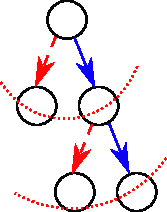
\includegraphics[width=25mm]{induction.pdf}
\end{center}
\end{minipage}
\caption{\label{fig-proof-ind} Proof by induction over the length of the path from the root to a node in the tree.}
\end{figure}

\paragraph{Providing witnesses:}
When reasoning about value ordering, it is common to use transitivity. For example, when searching for
a value in a search tree, we only compare the requested value with values stored along a single path in
the tree, that is, the path where it was expected to be stored. All other values are ruled out by
transitivity of the order relation. Unfortunately, due to how they handle universal quantification,
automatic provers used in \gnatprove are usually unable to come up with the appropriate
intermediate value to use in the transitivity relation. To achieve the proofs, we provided
provers with the appropriate term whenever necessary. For example, function \texttt{Find\_Root} in
Figure~\ref{fig-proof-wit} computes the first common ancestor of two nodes in a search tree. Indeed, as
the order invariant stated in Figure~\ref{fig-search} compares values on a single path, this
is the node to consider to be able to order values stored in arbitrary nodes.

\begin{figure}
% \begin{minipage}[c]{\linewidth}
\begin{small}
\begin{lstlisting}
function Find_Root (F : Forest; R, I, J : Index_Type) return Index_Type with
  Post =>
    --  The node returned is in the tree
    Model (F, R) (Find_Root'Result).Reachable

    --  The node returned is on the path of I
    and Model (F, R) (Find_Root'Result).Path <= Model (F, R) (I).Path

    --  The node returned is on the path of J
    and Model (F, R) (Find_Root'Result).Path <= Model (F, R) (J).Path

    --  The common ancestor of I and J is either I, or J, or an ancestor
    --  node such that the paths of I and J diverge at this point.
    and (I = Find_Root'Result
           or else J = Find_Root'Result
           or else Get (Model (F, R) (I).Path,
                        Length (Model (F, R) (Find_Root'Result).Path) + 1)
                /= Get (Model (F, R) (J).Path,
                        Length (Model (F, R) (Find_Root'Result).Path) + 1));
\end{lstlisting}
\end{small}
% \end{minipage}\hspace*{-30mm}
% \begin{minipage}[c]{.22\linewidth}
% \begin{center}
% 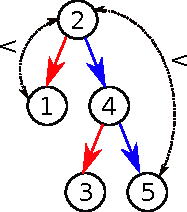
\includegraphics[width=28mm]{transitivity.pdf}
% \end{center}
% \end{minipage}
\caption{\label{fig-proof-wit} Function that computes a witness for transitivity applications.}
\end{figure}

% \paragraph{Case analysis:}
% As the number of cases to consider can sometimes confuse the prover, it is often useful to split the
% problem in a sensible way. A proof by case analysis is nothing more than an if statement, each branch
% narrowing the cases to consider and possibly providing additional informations on how to carry out
% the proof in this particular case. Figure~\ref{fig-proof-ca} shows how case analysis was used to
% prove how tree models are modified by an application of \texttt{Plug}. It is divided in two cases: either
% the node was already reachable from the root and then its model is unchanged, or it belonged to
% the subtree being plugged, in which case the path leading to it from the root consists in concatenating
% two subpaths.
%
% \begin{figure}
% \begin{small}
% \begin{lstlisting}
% --  Nodes have the same path in F_Old and F, or for those nodes
% --  for which V is on the path, their path is obtained by
% --  concatenating the path from R to V and the path from V to
% --  the node.
% for J in Index_Type loop
%
%    --  Case 1: node J is in the tree rooted at R in F_Old. Use
%    --  Preserve_Equal to prove the property for node J, based on
%    --  the knowledge that it holds for the parent of node J.
%
%    if Model (F, R) (J).Reachable
%      and then Length (Model (F, R) (J).Path) = N
%      and then Model (F_Old, R) (J).Reachable
%    then
%       Preserve_Equal (S1 => Model (F, R) (Parent (F, J)).Path,
%                       S2 => Model (F_Old, R) (Parent (F, J)).Path,
%                       S3 => Model (F, R) (J).Path,
%                       S4 => Model (F_Old, R) (J).Path,
%                       D  => F.C (J).Position);
%    end if;
%
%    --  Case 2: node J is in the tree rooted at V in F_Old. Use
%    --  Preserve_Concat to prove the property for node J, based
%    --  on the knowledge that it holds for the parent of node J.
%
%    if Model (F, R) (J).Reachable
%      and then Length (Model (F, R) (J).Path) = N
%      and then Model (F_Old, V) (J).Reachable
%      and then J /= V
%    then
%       Preserve_Concat (S1 => Model (F_Old, V) (Parent (F, J)).Path,
%                        S2 => Model (F, R) (Parent (F, J)).Path,
%                        S3 => Model (F_Old, V) (J).Path,
%                        S4 => Model (F, R) (J).Path,
%                        T  => Model (F, R) (V).Path,
%                        D  => F.C (J).Position);
%    end if;
%
%    --  Accumulate the knowledge that the property holds up to node
%    --  J.
%
%    pragma Loop_Invariant
%      (for all I in 1 .. J =>
%        (if Model (F, R) (I).Reachable and Length (Model (F, R) (I).Path) <= N then
%           (if Model (F_Old, R) (I).Reachable
%            then Model (F, R) (I).Path = Model (F_Old, R) (I).Path)));
%    pragma Loop_Invariant
%      (for all I in 1 .. J =>
%        (if Model (F, R) (I).Reachable and Length (Model (F, R) (I).Path) <= N then
%          (if Model (F_Old, V) (I).Reachable then
%             Is_Concat (Q => Model (F, R) (V).Path,
%                        V => Model (F_Old, V) (I).Path,
%                        P => Model (F, R) (I).Path))));
% end loop;
% \end{lstlisting}
% \end{small}
% \caption{\label{fig-proof-ca} Proof by case analysis of the effect of Plug on models.}
% \end{figure}
%
% Note that, to prove each cases, we use an intermediate lemma by calling the associated procedure (\texttt{Preserve\_Equal} and \texttt{Preserve\_Concat}).
% Also note that, to be able to apply this reasoning on every node of the memory array, the case
% analysis had to be enclosed in a loop. As \gnatprove cannot accumulated knowledge without a loop
% invariant, we had to restate everything that was proved so far by the loop as a loop invariant.
% Also note that this reasoning is a part of a reasoning by induction over the size \texttt{N} of the path
% leading to the node in the new tree, which is why we already know the proposition holds for the
% parent of the current node.

\subsection{Ghost Code}
% different uses of ghost code

% For specification purpose:
% - typically ghost functions used in contracts
% - can be interesting to execute as test oracles
% For verification purpose:
% - typically ghost procedures containing proofs by induction (loops), by case analysis...
% - no need to execute them, they do not bring anything
% No way to distinguish between both right now.

% factored out in ghost procedures to keep efficiency
% with or without contracts (inlining)

In this experiment, we made an extensive use of ghost code, that is, code meant only for verification,
that has no effect on the program behavior. We used it for two different purposes. First, the model
functions introduced to enhance the expressiveness of our specification are ghost functions. Indeed, we
never need to refer to reachability in the tree structure or to the set of elements contained in a
search tree inside the program implementation. It is only used to express complex
properties about our algorithms in the specification.

In SPARK, ghost code can be executable, that is, the compiler can be instructed to generate code for ghost
entities so that the contracts using them can be checked at runtime. In this spirit, ghost model functions
can be used to produce complex test oracles that can be exercised in the test campaign.

The second use of ghost code in our experiment is for auto-active verification. In particular, the procedures
used to encode intermediate lemmas are ghost, as they have no effect. What is more, we strived to
keep all verification-only code inside ghost procedures so that it can be removed by the compiler and will not
slow down the execution of the program. It is all the more important since the code is very inefficient, involving
multiple loops and model constructions. As functional behaviors are complex, coming up with contracts for
these ghost procedures can be painful, and produce huge, hard to read specifications. To alleviate this
problem, we can benefit from a feature of \gnatprove which inlines local subprograms with no contracts, allowing
the proof to go through with less annotation burden. In this way, we can choose, on a case-by-case basis, if
it is worthwhile to turn a chunk of auto-active proof into an intermediate lemma with its own contract,
allowing for a modular verification, or if we prefer to have the tool automatically inline the
proof wherever we call the ghost procedure.

% Note that, though it makes sense to execute ghost code used for subprogram specification, there is no benefit in
% executing code solely written for auto-active verification.

\section{Development and Verification Data}
% number of assertions, loc of ghost code, etc.
% data on automatic verification
% feedback from development and verification cycles

All the execution times and verification times reported in this section were
obtained on a Core i7 with 2,8 GHz and 16 GB RAM.

The code implementing the core algorithm for red-black trees, even when split
in three modules for binary trees, search trees and red-black trees, is quite
small, only 286 lines overall. But this code only accounts for 14\% of the
total lines of code, when taking into account contracts (22\%) and more
importantly ghost code (64\%). Table~\ref{tab-sloc} summarizes the logical
lines of code as counted by the tool GNATmetric.
% The imbalance would be even
% more pronounced if we looked at the effort required to produce the operational
% code, contracts and ghost code. The ratio for efforts would be closer to 9 to 1
% when comparing ghost code with operational code, as in the most complex cases
% developing ghost code required interacting with automatic provers to find a
% suitable division of proof objectives that was amenable to automatic proof.

\vspace{-0.5cm}
\begin{table}[h]
\begin{center}
\begin{tabular}{l|rrr|r}
                & code       & contracts  &      ghost  & total \\ \hline
binary trees    & 92  (10\%) & 250 (28\%) & 548  (62\%) & 890 \\
search trees    & 127 (12\%) & 188 (17\%) & 780  (71\%) & 1095 \\
red-black trees & 67  (52\%) & 18  (14\%) & 45   (35\%) & 130 \\ \hline
total           & 286 (14\%) & 456 (22\%) & 1373 (64\%) & 2115 \\
\end{tabular}
\vspace*{5mm}
\caption{\label{tab-sloc} Categorization of lines of code between operational code, contracts and ghost code.}
\vspace*{-10mm}
\end{center}
\end{table}

% There are few top-level contracts for red-black trees: just one precondition on
% the insertion procedure to state that there should be still room for insertion,
% and three postconditions on insertion, membership and the ghost function to get
% the set of values.
% Each of the contracts on red-black trees consists in just one
% conjunct, hence
% is only four.

%% As contracts can be arbitrarily complex, we prefer to count
%% the number of conjuncts than the number of preconditions and
%% postconditions.
There are few simple top-level contracts for red-black trees
(see Table~\ref{tab-sloc2}).  Many more
contracts and assertions are needed for auto-active verification, in the form
of subprogram contracts, type invariants, type default initial conditions, loop
invariants and intermediate assertions which split the work between automatic
provers and facilitate work of individual provers. The effort required to
achieve automatic proof is much greater where intermediate assertions are
needed, as more interaction with automatic provers is required in that case.

\vspace{-0.5cm}
\begin{table}[h]
\begin{center}
\begin{tabular}{l|rrrr|r}
                & on types & on subprograms & on loops & assertions & total \\ \hline
binary trees    & 10       & 155 (73)       & 42       & 12         & 219 \\
search trees    & 2        & 138 (60)       & 20       & 68         & 228 \\
red-black trees & 2        & 4 (4)          & 8        & 10         & 24 \\ \hline
total           & 14       & 297 (177)      & 70       & 90         & 471
\end{tabular}
\vspace*{5mm}
\caption{\label{tab-sloc2} Number of conjuncts (and-ed subexpressions) in contracts on types, on
  subprograms, in loop invariants and in assertions. Numbers in parentheses
  correspond to conjuncts for contracts on external subprograms.}
\vspace*{-10mm}
\end{center}
\end{table}

Taking both tables into account, it is clear that verification of search trees
was the most costly in terms of overall efforts, with a large part of ghost
code (71\%) and many intermediate assertions needed (68
conjuncts). Verification of red-black trees on the contrary was relatively
straighforward, with less ghost code than operational code (35\% compared to
52\%) and few intermediate assertions needed (10 conjuncts). This matches well
the cognitive effort required to understand the correction of search trees
compared to red-black trees.

The automatic verification that the code (including ghost code) is free of
run-time errors and that it respects its contracts takes less than 30 minutes,
using 4 cores and two successive runs
of GNATprove at proof levels 2 and 3. As automatic provers CVC4, Z3 and
Alt-Ergo are called in sequence on unproved Verification Conditions (VCs), it
is not surprising that CVC4 proves a majority of VCs (3763), while Z3 proves
103 VCs left unproved by CVC4 and Alt-Ergo proves the last 3 remaining VCs, for
a total of 3869 VCs issued from 2414 source code checks (1185 run-time checks,
231 assertions and 998 functional contracts).

As the code has been fully proved to be free of run-time errors and that all
contracts have been proved, it is safe to compile it with no run-time checks,
and only the precondition on insertion in red-black trees activated (since this
might be violated by an external call). Disabling run-time checks is done
through a compiler switch (-gnatp) and only enabling preconditions in red-black
trees is done through a configuration pragma in the unit. Inserting one million
integers in a red-black tree from 1 to 1 million leads to a violation of the
balancing in 999,998 cases, which requires 999,963 left rotations and no
right rotations. The running time for
performing these 1 million insertions is 0.65 seconds without run-time checks,
and 0.70 seconds with run-time checks, or 0.65 microseconds (respectively 0.70
microseconds) per insertion.

Enabling all contracts and assertions at run-time is also possible during
tests. Here, ghost code is particularly expensive to run, as constructing the
model for a binary tree is at worst quadratic in the size of the tree, and
contracts contain quantifications on the maximal size of the tree that call
functions which themselves quantify over the same size in their own contracts
or code. In addition, the expensive operation of constructing the model is
performed repeatedly in contracts, as SPARK does not yet provide a
let-expression form.  As a result, inserting one element in a tree of size one
takes 2 minutes.

\section{Related Work}
\label{related-work}
There have been several previous attempts at verifying red-black trees implementations. In particular, red-black trees are
used in the implementation of ordered sets and maps in the standard library of the Coq proof
assistant~\cite{appel2011efficient,filliatre2004functors}. As part of these libraries, the implementations have been proven
correct using interactive proofs in Coq. These implementations notably differ from our work because they are written in
a functional style, using recursive data types instead of pointers and recursive functions instead of loops. Similar
libraries are provided for the Isabelle proof assistant~\cite{lammich2010isabelle}. Functional implementations of
red-black trees have also been verified outside of proof assistants, using characteristic formulas~\cite{chargueraud2010program},
or in the Why3 programming language as part of VACID-0 competition~\cite{leino2010vacid}. This last implementation differs from
the previous ones in that it is mostly auto-active, even if it uses Coq for a few verification conditions.

Verifying imperative implementations of red-black trees is more challenging as it involves reasoning about the well-formedness
of the tree structure, which comes for free in the functional implementations. As part of VACID-0, attempts have been made at
verifying red-black trees in C using VCC and in Java using KeY~\cite{bruns2011specification}.
Both attempts seem to have been left in preliminary stages
though.
%%  as the Java version only focuses on expressing the invariants, without attempting to verify them, while the C
%% version only verifies properties relative to the well formedness of their tree structure.

More recently, imperative implementations of red-black trees in C and Java have been verified using more specialized logics.
Enea et al. obtained an automatic verification of a C implementation of red-black trees using separation logic, a logic
specialized for the verification of heap manipulating programs~\cite{enea2015automated}. In the
same way, Stef{\u{a}}nescu et al. were able to verify several implementations of red-black trees in particular in Java and
C using matching logic~\cite{stefuanescu2016semantics}. As used in this work, matching logic provides a very precise,
low-level view of the heap structure, allowing for powerful proofs on this kind of programs. Both works use specialized tools,
which are specifically designed for verifying low-level, heap manipulating programs but which have never been used, to the best
of our knowledge, to verify higher-level software.

\section{Conclusion}
In this article, we have explained how, using auto-active techniques, we could achieve formal verification of key functional
properties of an imperative implementation of red-black trees in SPARK. This is not an example of what should be a regular
use of the SPARK toolset but rather a successful demonstration of how far we can go using such technology.

However, the techniques presented on this example can be reused with significant benefits on a much smaller scale. In particular, we have shown that
inductive proofs can be achieved rather straightforwardly using auto-active reasoning. The multi-layered approach, using
type invariants and model functions to separate concerns, can also be reused to reason about complex data structures.

To popularize the use of auto-active techniques, we are also working on integrating simple interactive proof capabilities
in GNATprove. This would allow applying the same techniques in a simpler, more straightforward way, and also to avoid
polluting the program space with ghost code which is never meant to be executed.

\paragraph*{Acknowledgements.}
We would like to thank the anonymous reviewers for their useful comments.


\bibliographystyle{splncs03}
\bibliography{nfm_2017}

\end{document}
